\begin{problem}{三年坂二年坂}{三年坂二年坂.in}{三年坂二年坂.out}{1 seconds}

八百比丘尼五一的时候带着晴明和博雅来到京都最有名的商业街---三年坂二年坂游玩,琳琅满目的商品让博雅看花了眼,但是由于晴明在和八岐大蛇的战斗中身受重伤,刚复原不久,不宜过度耗费体力,因此他们决定用他们身上有限的T日元去购买商业街上的商品,已知商业街上一共有N家商店,每家商店有$a_{i}$($1 \leq i \leq N$)日元的商品,现在要求你计算出在保证正好花光T日元的前提下,把M家商店的东西都买完\textbf{(假设编号k家商店的商品一共是$a_{k}$元,如果三人选择购买此家商品,必须把$a_{k}$元的商品全部买走ORZ)},请问,M最小值是多少?\textbf{(要求这M家商店是相连的)}如果不存在这样的M家商店,输出“No”,反之输出M。

\begin{center}
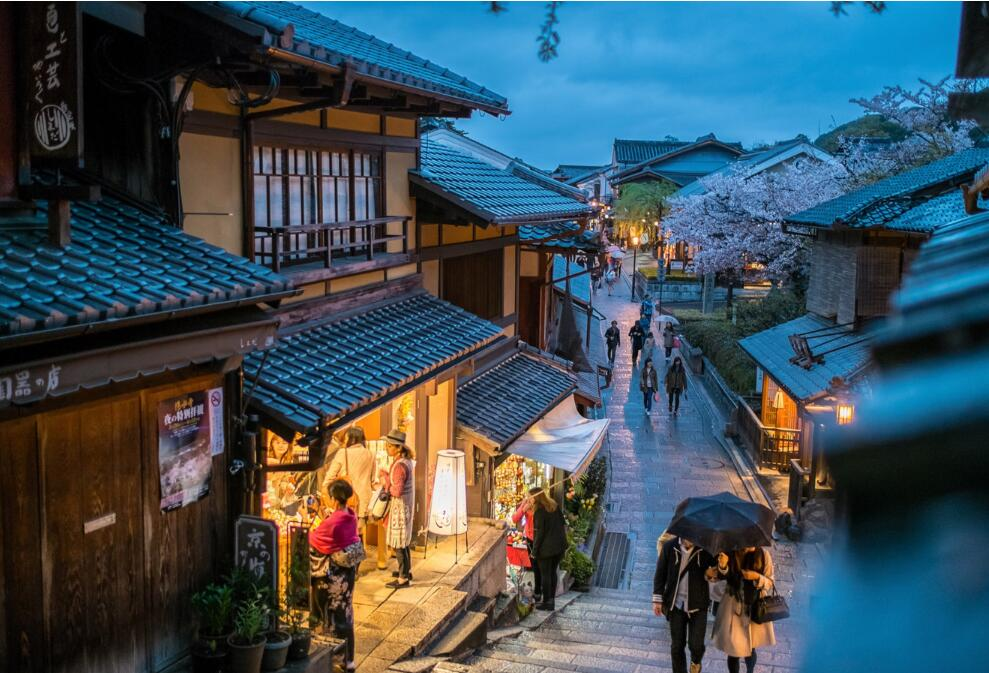
\includegraphics[width=0.8\textwidth]{pics/D.jpg}
\end{center}

\InputFile

第一行输入两个正整数N和T表示商店的数目和三人所能使用的日元总额($1 \leq N \leq 1e5,1 \leq T \leq 1e8$)
 
接下来输入N家商店对应的物品价值$a_{i}$($1 \leq a_{i} \leq 1e4$)

\OutputFile

输出符合条件的最小商店的数目M,如不存在输出“No”

\Example

\begin{example}
\exmp{
10 15
5 1 3 5 10 7 4 9 2 8
}{
2
}%
\exmp{
5 11
1 2 3 4 5
}{
No
}%
\end{example}

样例1:选第4家店(5)和第5家店(10),15=5+10

样例2:没有符合要求的M家商店

\end{problem}
